\documentclass[12pt]{article}
\usepackage{amsmath}
\usepackage{amssymb}
\usepackage{geometry}
\usepackage{enumerate}
\usepackage{natbib}
\usepackage{float}%稳定图片位置
\usepackage{graphicx}%画图
\usepackage[english]{babel}
\usepackage{a4wide}
\usepackage{indentfirst}%缩进
\usepackage{enumerate}%加序号
\usepackage{multirow}%合并行


\begin{document}
\newpage
\section{Problem 1}
\subsection{(a)}
$$A_v=-\sqrt{\frac{\mu_n(W/L’)_1}{\mu_p(W/L‘)_2}}$$
$$-5=-\sqrt{\frac{350(x/2)}{100(5/2)}}$$
$$x=35.7\mu m$$
$$V_{TH}=0.7V$$
$$\mu_nC_{ox}(\frac{W}{L})_1(V_{in1}-V_{TH1})^2=\mu_pC_{ox}(\frac{W}{L})_2(V_{DD}-(V_{in1}-V_{TH1})-V_{TH2})^2$$
$$0.035*\frac{35.7}{2-2*0.08}*(V_{in1}-0.7)^2=0.01*\frac{5}{2-2*0.09}*(5-(V_{in1}-0.7)-0.8)^2$$
$$V_{in1}=1.4V$$
The range for $V_{in}$ is (0.7, 1.4)V.
\subsection{(b)}
\begin{figure}[H]
\centering
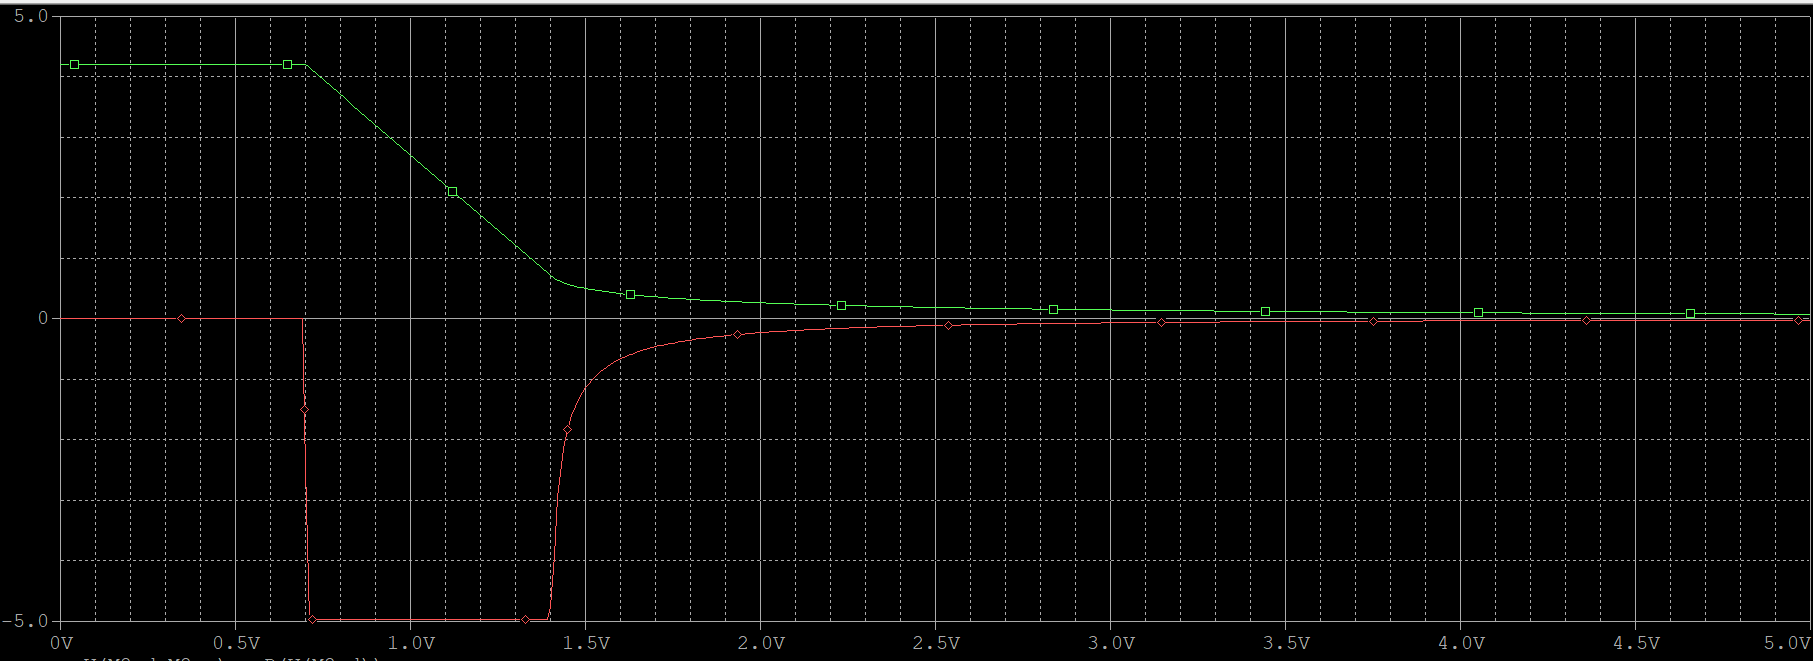
\includegraphics[scale=0.25]{P1.png}
\end{figure}
This is the plot of $V_{out}$ and $A_v$ vs $V_{in}$, when $V_{in}$ is about 1V, $A_v$ is very close to the calculated value, and the the $V_{out}$ is in saturation region when $V_{in}$ is in my calculated region.
\subsection{(c)}
\begin{figure}[H]
\centering
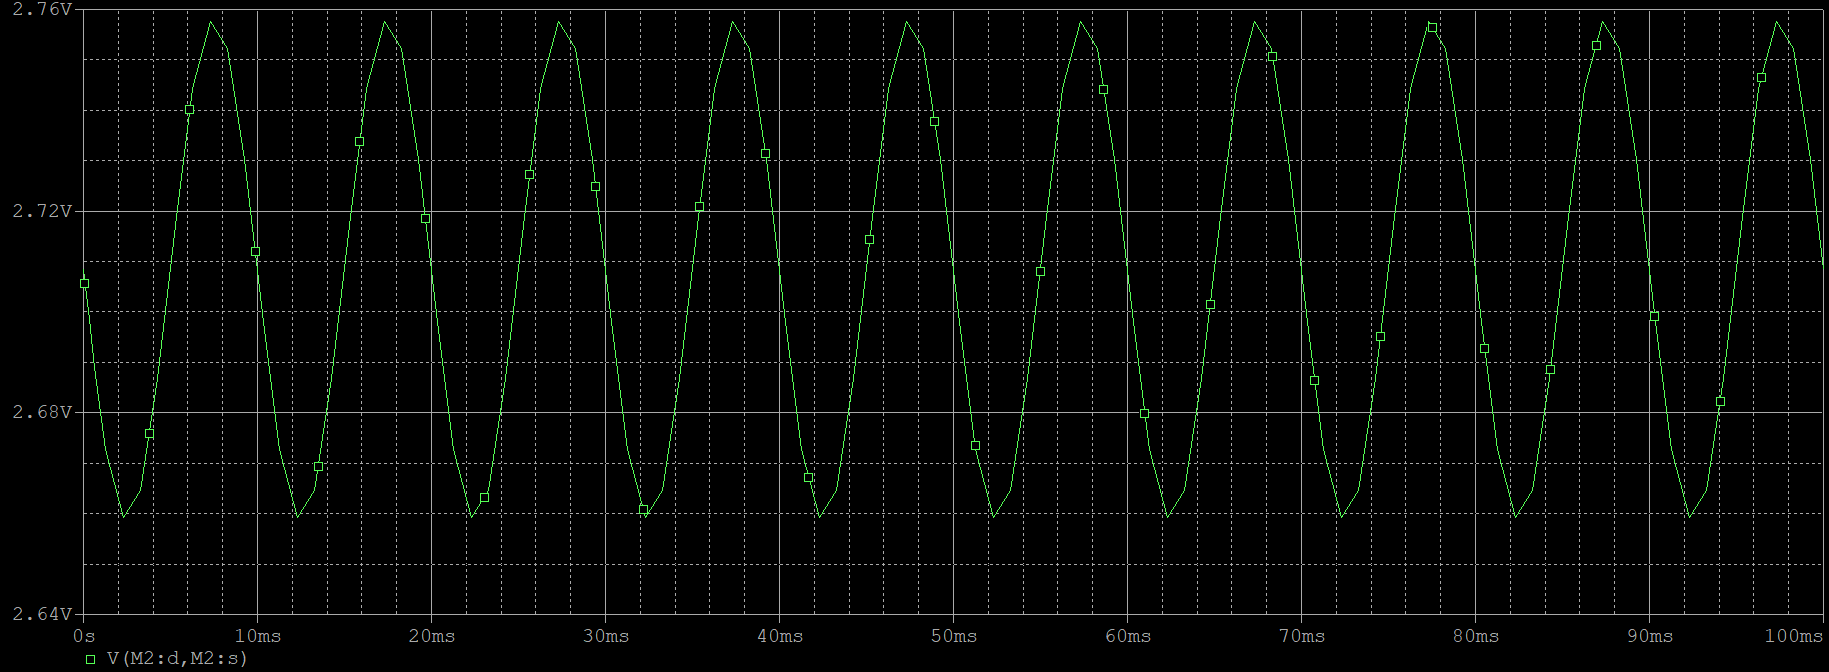
\includegraphics[scale=0.25]{P2.png}
\caption{$V_{in}$ has amplitude 0.01V}
\end{figure}
\begin{figure}[H]
\centering
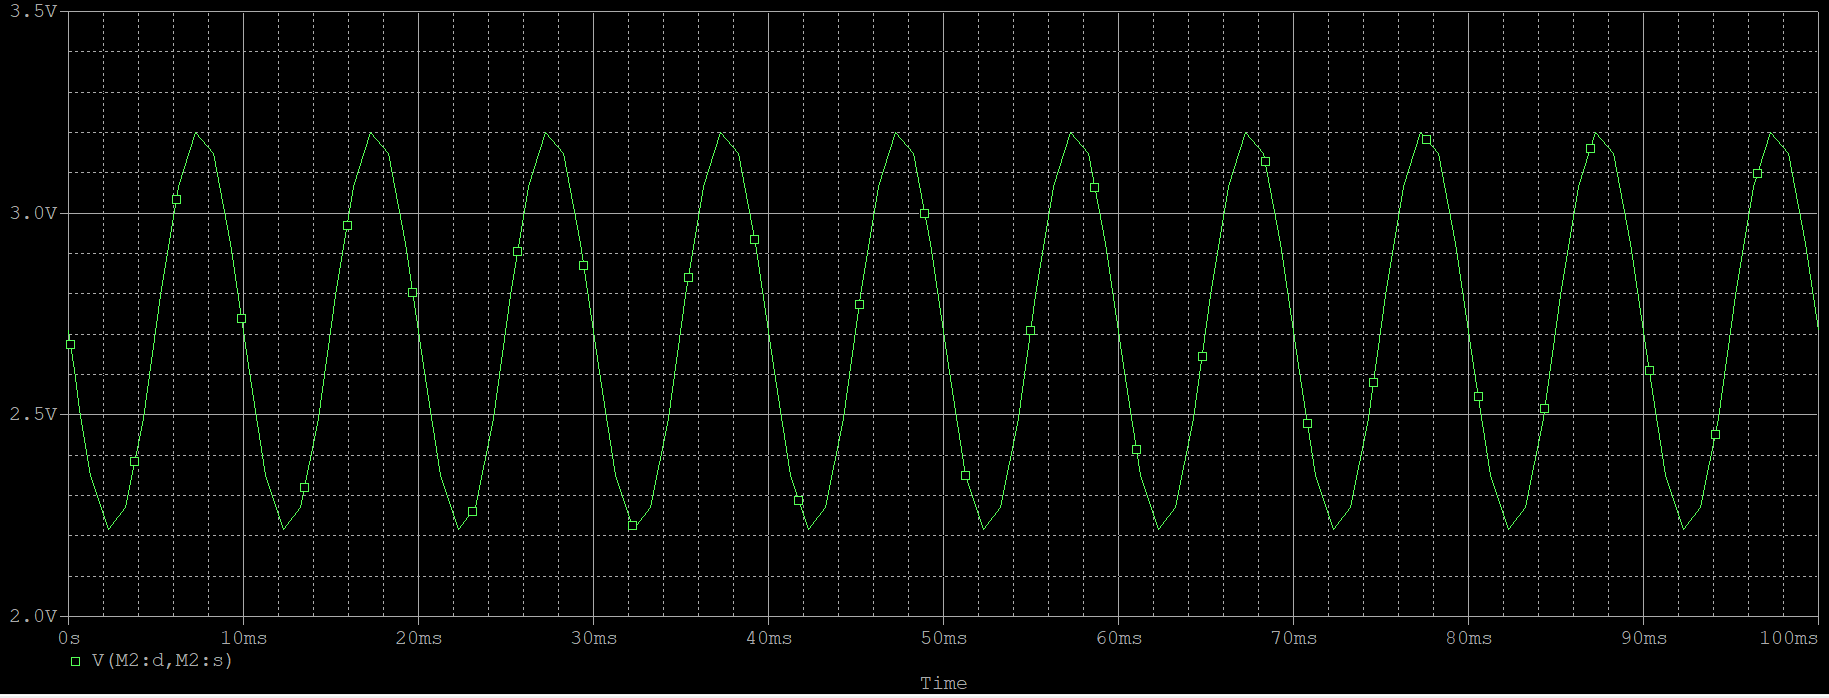
\includegraphics[scale=0.25]{P3.png}
\caption{$V_{in}$ has amplitude 0.1V}
\end{figure}
\begin{figure}[H]
\centering
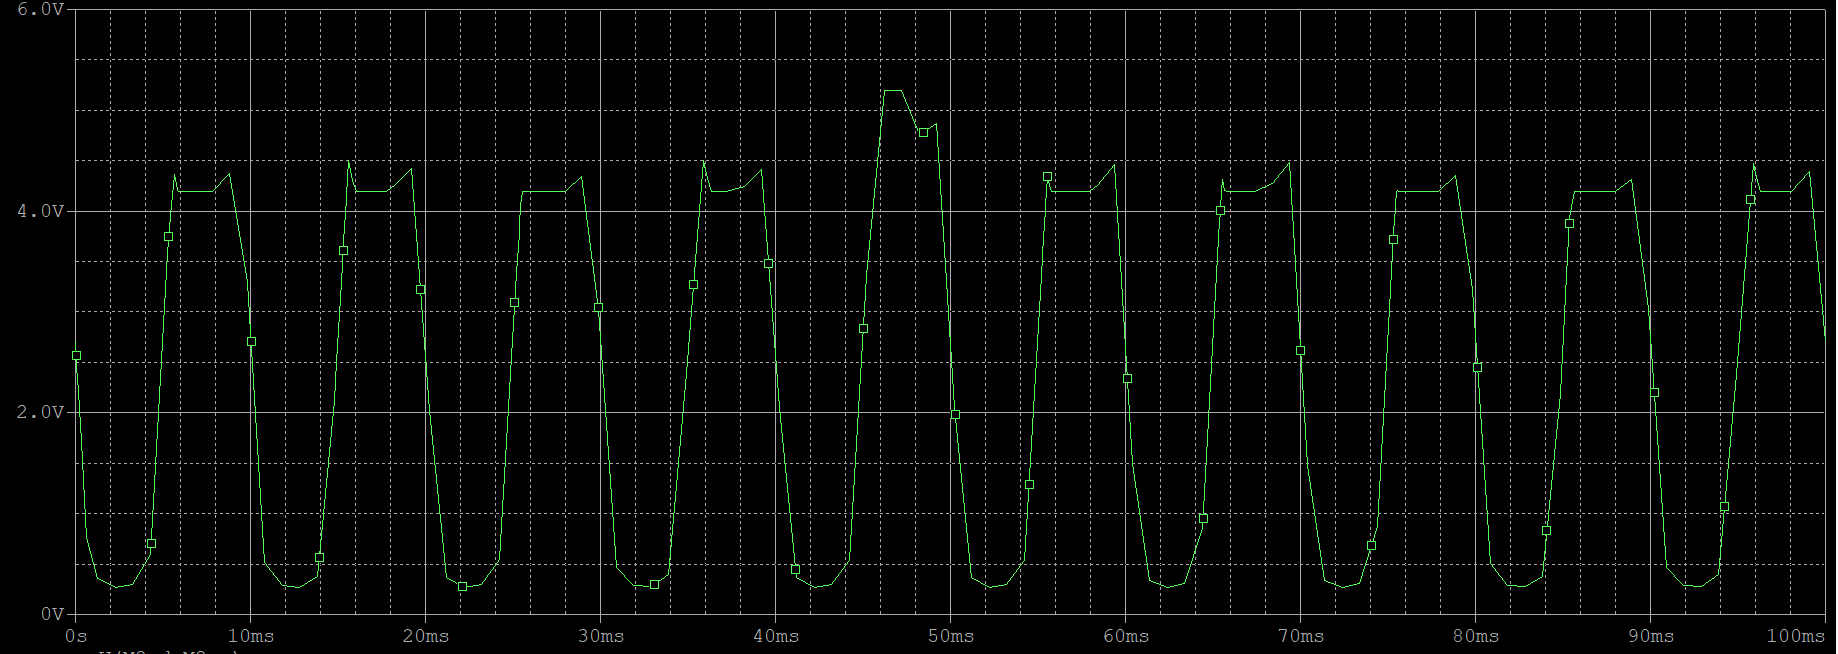
\includegraphics[scale=0.25]{P4.png}
\caption{$V_{in}$ has amplitude 1V}
\end{figure}
In Figure 3, the $V_{in}$ is so large so that the nmos is no longer in saturation region, then it seems the upper part of the plot has been cut off
\section{Problem 2}
\subsection{(a)}
For the circuit, assume $V_{out}>V_{in}-V_{TH}$
$$V_{out}=V_{DD}-I_cR_D=5-100000I_c$$
$$I_c=\frac{1}{2}\mu_nC_{ox}(\frac{W}{L})_1(V_{in1}-V_{TH1}-I_cR_s)^2=7.3\times10^{-3}*(V_{in}-0.7-20000I_c)^2$$
$$A_v=\mathbf{\frac{dV_{out}}{dV_{in}}}=\mathbf{\frac{\frac{dV_{out}}{dI_c}}{\frac{dV_{in}}{dI_c}}}=\frac{-100000}{20000+5.85*I_c^{-0.5}}$$
When $V_{in}=1.2V$, $I_c=2.81\times10^{-5}(A)$
$$A_v=\mathbf{\frac{dV_{out}}{dV_{in}}}=\frac{-100000}{20000+1103.5}=-4.7$$
$$gm_1=\mu_nC_{ox}(\frac{W}{L})_1(V_{in1}-V_{TH1})^2=0.035*\frac{3.9*8.85*10^{-12}}{9*10^{-9}}*\frac{200}{2-2*0.08}*(1.2-0.7)^2=3.65\times10^{-3}$$
Since $\lambda=0$, then $r_{o1}=\infty$. Also $\gamma=0$, then $gm_1=0$, so the voltage gain will become 
$$A_v=-\frac{R_{D}}{R_{S}}=\frac{100}{20}=5$$
The to $A_v$ are very close to each other.
\subsection{(b)}
\begin{figure}[H]
\centering
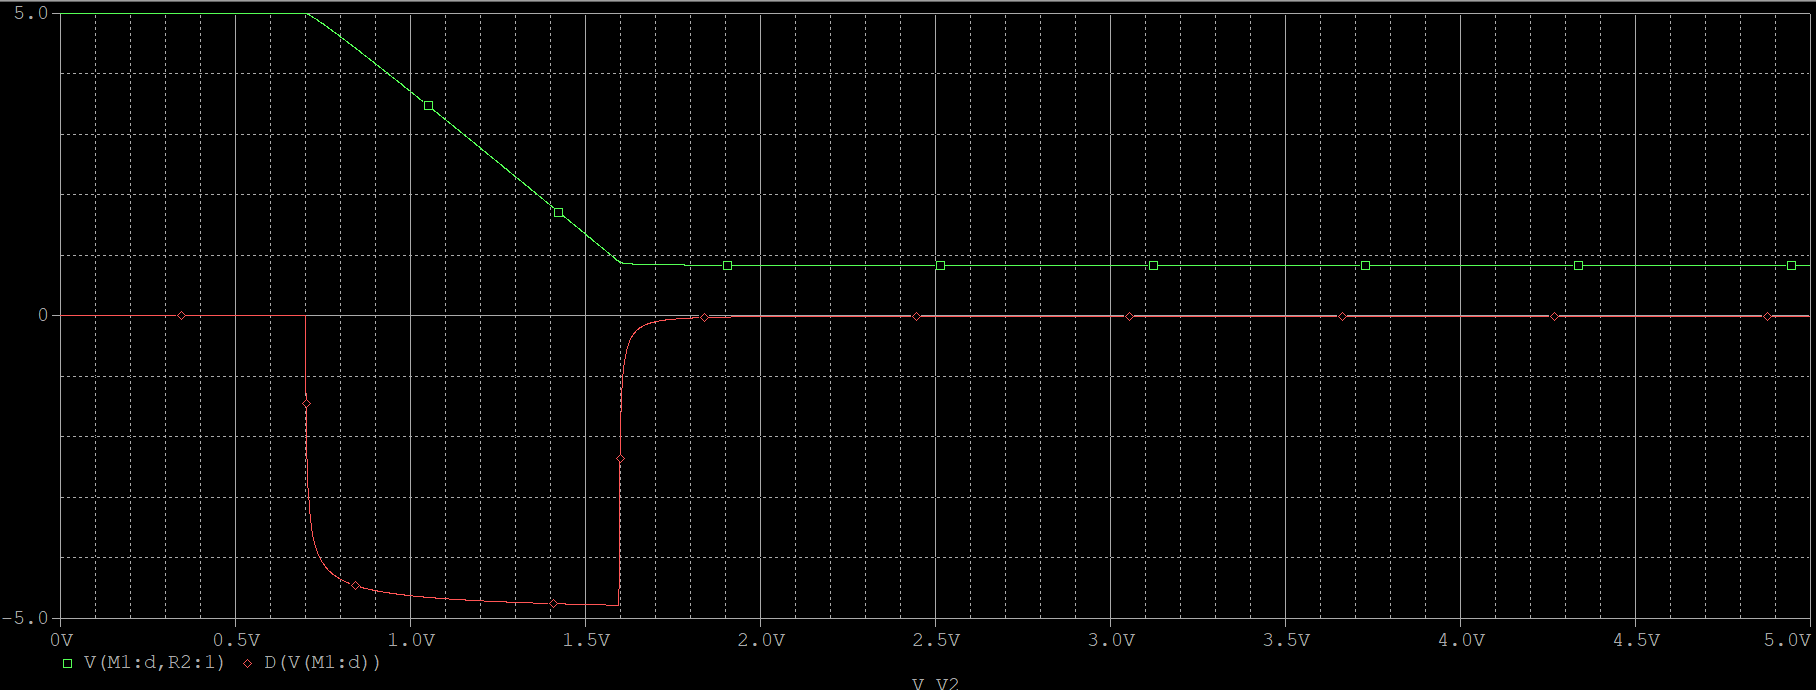
\includegraphics[scale=0.25]{P5.png}
\end{figure}
This is the plot of $V_{out}$ and $A_v$ vs $V_{in}$, when $V_{in}$ is about 1.2V, $A_v=-4.7$, which is very close to the calculated value.
\subsection{(c)}
\begin{figure}[H]
\centering
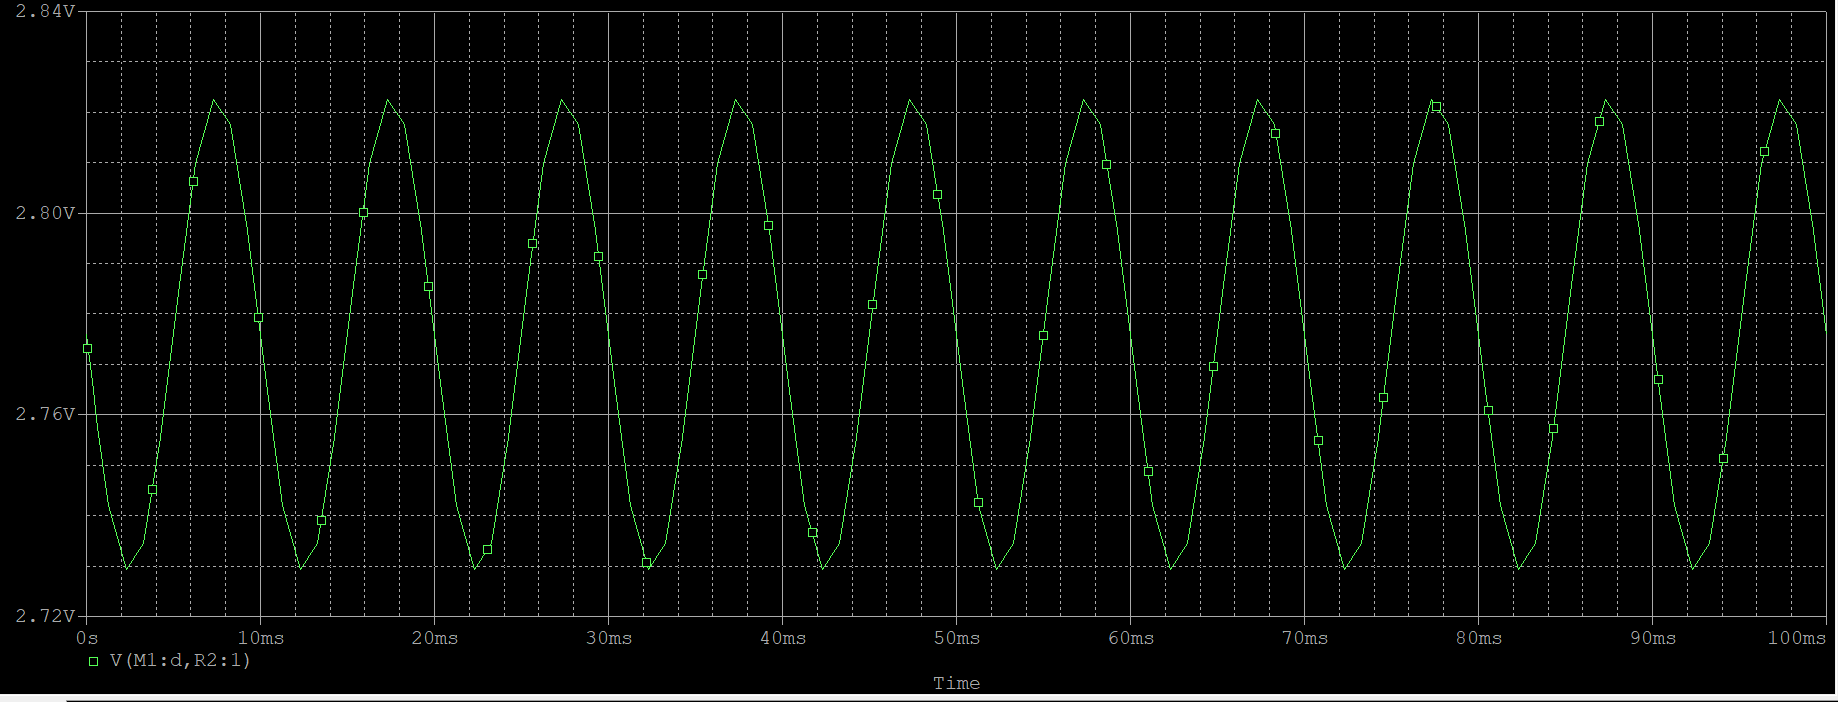
\includegraphics[scale=0.25]{P6.png}
\caption{Plot of $V_{out}$ vs $t$}
\end{figure}
\end{document}